\documentclass[10pt,a4paper]{article}
\usepackage[textwidth=16cm,textheight=23cm]{geometry}
\usepackage[utf8]{inputenc}
\usepackage[T1]{fontenc}
\usepackage{amsmath}
\usepackage{amsfonts}
\usepackage{amssymb}
\usepackage{graphicx}
%\usepackage{url}
\usepackage{hyperref}

\newcommand{\Trans}{\mathcal{T}}
\newcommand{\filterationF}{\mathcal{F}}
\newcommand{\mkt}{\mathrm{mkt}}
\newcommand{\ytw}{\mathrm{ytw}}
\newcommand{\dd}{\mathrm{d}}
\newcommand{\CRdelta}{\mathrm{CR01}}

\parindent=0pt
\parskip=1.5ex


\begin{document}

\title{Note on Callable Bonds}
\author{Youngsuk Lee}
\date{20 May 2020}
\maketitle

\section{Structure: Callable Bonds}

Consider a callable bond with call dates at
\begin{equation}
T_1 < T_2 < \cdots < T_M
\end{equation}
If the issuer calls, or {\em redeems}, the bond on $T_m$, the redemption amount and the outstanding accrued interest is paid to the bond holder at $T_m$ and the remaining cash flows are cancelled. Here, for convenience, the maturity date is treated as the last call date $T_M$. 


Typically (at least in old days), callable bonds are structured so that it is most economical for the issuer to redeem on the first call date. For example, the coupon payments after the first call are based on Libor plus very large spread. In past, when callable bonds were not redeemed on the first call date, such events were surprise news to the market. 
\begin{itemize}
	\item Deutsche Bank non-call, Dec 2008: \href{https://in.reuters.com/article/deutsche-bank-bond-call/update-2-deutsche-bank-non-call-casts-shadow-over-lt2-bonds-idINLH25709820081217}{Reuters news}
	\item Woori Bank, Feb 2009: \href{https://www.reuters.com/article/woori-bonds/asia-credit-woori-bank-seen-calling-back-400-mln-of-debt-idUSHKG35800620090209}{Reuters news}
	\item Monte dei Paschi di Sienna, Feb 2011:
	\href{https://ftalphaville.ft.com/2011/02/17/491236/another-bank-non-call-an-entirely-different-reaction/}{Financial Times Alphaville}
\end{itemize}

\section{Pricing Models}

\subsection{Yield-to-Worst Pricing Model}
\label{sec:pricing-model-yield-to-worst}

\subsubsection{Yield-to-Worst}
\label{sec:yield-to-worst}

A widely-used pricing model is to search for the call date which results in the worst yield from the investor's perspective (or the best yield from the issuer's perspective), i.e.\ the smallest yield. 

Being precise, let
\begin{itemize}
	\item $\bar{V}$: the market value of the bond with the unit principal on the calculation date
	\item $V_m(y)$: the present value, in terms of yield-to-maturity $y$, of the underlying-bond associated with call date $T_m$: 
	\begin{equation}
	V_m(y) = \sum_{t_j \le T_M} c_j  e^{-yt_j} + N_m e^{-yT_m}
	\label{eqn:valuation-non-callable-bond}
	\end{equation}
	where $c_j$ is the coupon amount paid on $t_j$ and $N_m$ is the redemption amount. 
\end{itemize}
In practice, $c_j$ depends on a floating rate (e.g.\ Libor) after the first call date. But, for discussion purposes, we simply assume it is fixed. 

To calculate the yield-to-worst $\bar{y}$, 
\begin{enumerate}
	\item For each $m = 1, \cdots, M$, solve the following equation to get the yield-to-maturity $\bar{y}_m$ for the $m$-th call date:
	\begin{equation}
	V_m(\bar{y}_m) = \bar{V}
	\end{equation}
	\item $\bar{y}$ is set to
	\begin{equation}
	\bar{y} := \min_m \bar{y}_m, \quad m = 1, \cdots, M
	\end{equation}
\end{enumerate}

Equivalently, the yield-to-worst $\bar{y}$ is the solution for the following equation:
\begin{equation}
\min_{m} V_m(y) = \bar{V}, \quad m = 1, \cdots, M
\end{equation}
To prove this, we have, by definition, 
\begin{equation}
\bar{V} = V_m(\bar{y}_m) \le V_m(\bar{y})
\end{equation}
Taking $\min$, 
\begin{equation}
\bar{V} \le \min_m V_m(\bar{y})
\end{equation}
Find $\bar{m}$ such that $\bar{y} = \bar{y}_{\bar{m}}$. Then, we have
\begin{equation}
\bar{V} \le \min_m V_m(\bar{y}) \le V_{\bar{m}}(\bar{y}_{\bar{m}}) = \bar{V}
\end{equation}
Now, we are ready to formally define the yield-to-worst pricing model. 

\subsubsection{Formal Definition}
\label{sec:ytw-formal-def}

{\bf Definition}: The {\em yield-to-worst pricing model} is a valuation model where the bond valuation is defined by the following function $V$ in terms of a yield $y$:
\begin{equation}
V(y) = \min_m V_m(y), \quad m = 1, \cdots, M
\label{def:pricing-model-yield-to-worst}
\end{equation}

For a given market value $\bar{V}$, 
\begin{itemize}
	\item $\bar{y}$: the yield, referred to as {\em yield-to-worst}, for the callable bond satisfying $V(\bar{y}) = \bar{V}$
	\item $\bar{y}_m$: the yield for the $m$-th non-callable bond such that $V_m(\bar{y}_m) = \bar{V}$.
	\item $\bar{m}$: the index of the call date at which the minimum in (\ref{def:pricing-model-yield-to-worst}) is achieved, {\em assuming} that a unique such call date exists. Under this assumption, we have
	\begin{equation}
	\bar{y} = \bar{y}_{\bar{m}}
	\end{equation}
	If the assumption is invalid, $\bar{m}$ is ill-defined. 
\end{itemize}

If $\bar{m}$ is uniquely well-defined, the underlying bond associated with call date $T_{\bar{m}}$ is referred to as the {\em yield-to-worst} bond. Because of its simplicity, the YTW bond is often used as the starting point for analysing the actual callable bond. 

\begin{figure}[h!]
	\begin{center}
	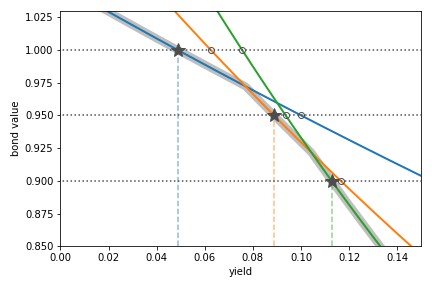
\includegraphics[width=10cm]{pics/pv-ytw.png}
	\end{center}
	\caption{
		[thick grey line]: value profile for the callable bond example in Section \ref{sec:ytw-formal-def}. [blue/orange/green solid lines]: value profiles for its 1st/2nd/3rd underlying bonds, respectively. 
		[dotted lines]: three market value scenarios at 1.0,conditions 0.95 and 0.9.
		[dashed lines]: yields-to-worst implied from the valuation model  (\ref{def:pricing-model-yield-to-worst}) for the three market value scenarios. The colours match to the worst-to-yield underlying bond. [stars/circles]: yield/market-value pairs implied from the non-callable valuation model (\ref{eqn:valuation-non-callable-bond}) of the underlying bonds for the scenarios. The pairs associated with yields-to-worst are marked with stars and others with circles.}
	\label{fig:pv-ytw}	
	\hrule
\end{figure}

To demonstrate the concept using graphs, consider a callable bond with the following structure:
\begin{itemize}
	\item coupon schedule: three annual coupons with
	$$\{(t_j, c_j)\}_{j=1}^{3} = \{(1,0.05), (2,0.08), (3,0.11) \}$$
	\item call dates: $T_1 = 1$, $T_2 = 2$ and $T_3 = 3$ with $M=3$. Recall that $T_M$ is the maturity date. 
	\item redemption amount: $1$
\end{itemize}


Figure \ref{fig:pv-ytw} should the value profiles of the callable bond itself (thick grey line) and its three underlying bonds (coloured lines). Three scenarios of the market value are considered with the following observations
\begin{center}
	\begin{tabular}{cccc}
		\hline
		scenario of market value & yield-to-worst & $\bar{m}$ \\
		\hline
		1.0  & 0.04879017 & 1\\
		0.95  & 0.08880587 & 2\\
		0.9  & 0.11273707 & 3\\
		\hline
	\end{tabular}
\end{center}


\subsubsection{P\&L Explain using Yield-to-Worst Bond}

The purpose of this section is to discuss the validity of the YTW bond as an approximation to the callable bond. 

If $y$ is sufficiently close to $\bar{y}$, the minimum in (\ref{def:pricing-model-yield-to-worst}) will be achieved at $\bar{m}$ as well. Thus, the callable bond can be valued using the YTW as well: 
\begin{equation}
V(y) = V_{\bar{m}}(y)
\end{equation}
for $|y - \bar{y}| < \epsilon$ for some $\epsilon > 0$. Therefore, 
\begin{itemize}
	\item The YTW bond model $V_{\bar{m}}(y)$ can be used to calculate any sensitivities of the full model $V(y)$ at $\bar{y}$ and the calculation is {\em exact} without any approximation:
	\begin{equation}
	\frac{\dd^k V}{\dd y^k}(\bar{y}) = \frac{\dd^k V_{\bar{m}}}{\dd y^k}(\bar{y})
	\end{equation}
	\item Consequently, any Taylor expansion to the callable bond can be calculated {\em exactly} using the YTW bond. For example, the first-order expansion is given by
	\begin{equation}
	V(y) - V(\bar{y}) \approx \frac{\dd V_{\bar{m}}}{\dd y}(\bar{y})(y - \bar{y})
	\end{equation}
\end{itemize}


If, however, $y$ is not sufficiently close enough from $\bar{y}$, i.e.\ $|y-\bar{y}| \gg \epsilon$, the minimum in (\ref{def:pricing-model-yield-to-worst})
may be achieved in $m' \ne \bar{m}$, i.e.\
\begin{equation}
V(y) = V_{m'}(y)
\end{equation}
Then, any analysis based on the YTW bond becomes invalid. 

To illustrate the above discussions, Figure \ref{fig:error-ytw} shows the error profile $e(y)$ when the callable bond is approximated using the yield-to-worst bond:
\begin{equation}
e(y) = V(y) - V_{\bar{m}}(y)
\end{equation}
The three scenarios in Figure \ref{fig:pv-ytw} are considered. 
For each scenario, the error is exactly zero if the yield is near the yield-to-worst, but becomes significantly negative as the yield gets away from it. 

\begin{figure}[h!]
	\begin{center}
		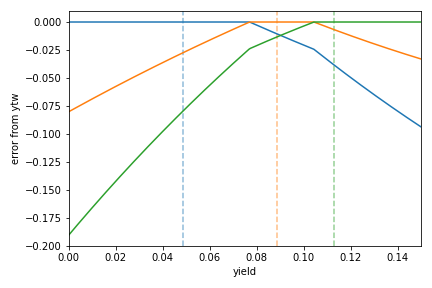
\includegraphics[width=10cm]{pics/error-profile-ytw.png}
	\end{center}
	\caption{
		[dashed lines]: Yields-to-worst corresponding to the three scenarios in Figure \ref{fig:pv-ytw}. 
		[solid lines]: Error profiles when the yield-to-worst bond valuation model is used. Each line corresponds to each of three market scenarios.}
	\label{fig:error-ytw}
\end{figure}


Summarising, 
\begin{itemize}
	\item The YTW bond model $V_{\bar{m}}(y)$ is exact to the callable-bond model $V(y)$ {\em only} for $y$ sufficiently close to $\bar{y}$.
	\item In general, the full revaluation must be adopted in order to calculate the change in value of the callable bond, 
	\begin{equation}
	V(y) - V(\bar{y}) = \min_m V_m(y) - \min_m V_m(\bar{y})
	\end{equation}
\end{itemize}
Finally, if there are more than one candidates for $\bar{m}$, one cannot define a YTW bond. Thus, any arguments based on a YTW bond are completely invalid 

\subsubsection{Optionality and Option Value}

It is important to notice that, with the Yield-to-Worst pricing model in Eq (\ref{def:pricing-model-yield-to-worst}), 
\begin{itemize}
	\item the optionality is captured as the minimum operator is applied across all potential underlying bonds
	\item the option value is zero because the exercise decisions are deterministically decided. In order to have non-zero option value, a stochastic model such as described in Section \ref{sec:pricing-model-stochstic-yield} should be considered. 
\end{itemize}

\subsection{Stochastic Yield Pricing Model}
\label{sec:pricing-model-stochstic-yield}

The model described in Section \ref{sec:pricing-model-yield-to-worst} is deterministic where bond yields in future are completely determined from the today's yield. This is not a realistic assumption. Thus, an {\em stochastic yield} (SY) pricing model should be considered
\begin{equation}
P(y) = E\left[ V(Y) \right]
\end{equation}
where $Y$ is a random variable representing the distribution of possible future yields. Because of the $\min$ operator in $V(y)$, we expect to have negative option value: 
\begin{equation}
P(y) - V(y) \le 0
\label{eqn:option-value}
\end{equation}
This is in line with the fact that the investors {\em short the option} as the call right is with the issuer. 

Whilst it is outside the scope of this document how $Y$ is modelled, its volatility would be calibrated to market variables such as swaption volatilities. Thus, being precise, the SY model should be written as
\begin{equation}
P(y) = P(y, \sigma)
\end{equation}
where $\sigma$ indicates the dependence on, say, swaption volatilities. 

The most notable effect of introducing stochastic nature in the yield dynamics is to smooth out the kinks from the deterministic model as illustrated in Figure \ref{fig:pv-sy}.\footnote{Here, we used the following simple model for $Y$:
\begin{equation}
Y \sim N(y, \nu^2)
\end{equation}
with $\nu = 0.03$.}
Notably, the first-order sensitivity becomes continuous (and smooth) as shown in figure (c). Finally, the error profiles are shown in figure (d) when the YTW bond is used to approximate the SY model. 


\begin{figure}[h!]
	\begin{center}
		\begin{tabular}{cc}
			(a) bond value & (b) option value \\
		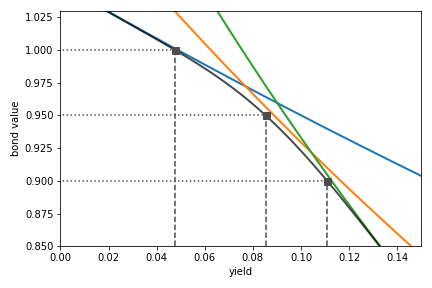
\includegraphics[width=7cm]{pics/pv-sy.png}
		&
		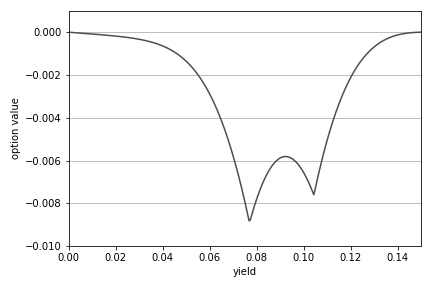
\includegraphics[width=7cm]{pics/option-value.png}
		\end{tabular}
	
		\begin{tabular}{cc}
			(c) first-order sensitivity & (d) error from yield-to-maturity bond\\
			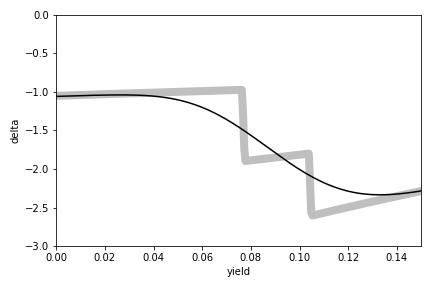
\includegraphics[width=7cm]{pics/delta.png}
			&
			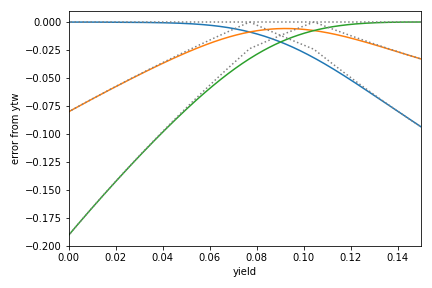
\includegraphics[width=7cm]{pics/error-profile-sy.png}
		\end{tabular}
		
	\end{center}

	\caption{
		The same callable bond example and three market value scenarios described in Figure \ref{fig:pv-ytw} are considered. 
		(a) [black line]: SY yield model $P(y)$ as a function of yield. 
		[coloured lines]: The same lines in Figure \ref{fig:error-ytw}. 
		[squares]: yield/value pairs implied from the SY pricing model for each scenario.
		(b) Option-value per (\ref{eqn:option-value}): difference between the black line in Figure (a) and the thick grey line in Figure \ref{fig:pv-ytw}.
		(c) First-order sensitivity profiles from the yield-to-worst model (thick grey line) and the SY yield model (think black line). 
		(d) [solid lines]: Error profiles when the yield-to-worst bond valuation model is used. [dotted lines]: Taken from Figure \ref{fig:error-ytw} for comparison.
		}
	\label{fig:pv-sy}
\end{figure}


\subsection{Spread-to-Worst Pricing Model}

Instead of searching for the worst yield, one can search for the worst spread $s$ over a given benchmark interest rate curve $r(t)$:
\begin{equation}
V(s, r(t)) := \min_m V_m(s, r(t))
\end{equation}
where
\begin{equation}
V_m(y, r(t)) = \sum_{t_j \le T_M} c_j  e^{-(r(t_j) + s)t_j} + N_m e^{-(r(t_j) + s)T_m}
\label{eqn:valuation-non-callable-bond-spread}
\end{equation}


\subsection{Stochastic Spread Pricing Model}

Similar to the Stochastic Yield Pricing Model, we consider a random variable $S$ for future spreads over a given benchmark interest rate curve $r(t)$:\footnote{Here, only $s$ is simulated. In addition, $r(t)$ could be simulated as well.}
\begin{equation}
P(s, r(t)) := E\left[V(S,r(t))\right].
\end{equation}


\section{Summary}


Avoid YTW Pricing Model:
\begin{itemize}
	\item We should avoid using the YTW pricing model because the profile is not smooth with kinds.
	\item If the YTW pricing model is the only available option, one should not use the underlying YTW bond because
	\begin{itemize}
		\item Such a bond may be well-defined to begin with. 
		\item It can change from one to another as the market changes, making any temporal analysis unstable. 
		\item For large market changes, the YTW bond becomes a bad approximation to the original callable bond. Instead, one must use the full pricing model (\ref{def:pricing-model-yield-to-worst}). 
	\end{itemize}	
\end{itemize}
Equally, we should avoid Spread-to-Worst pricing model. 


Use a stochastic model (e.g.\ Stochastic Yield or Spread model) instead:
\begin{itemize}
	\item This will smooth out the value profile. Consequently, all sensitivities are well-defined. 
	\item For large market changes, we have to perform full-revaluations as the value profiles are highly non-linear.  
\end{itemize}


\end{document}